%%%%%%%%%%%%%%%%%%%%%%%%%%%%%%%%%%%%%%%%%
% Beamer Presentation
% LaTeX Template
% Version 1.0 (10/11/12)
%
% This template has been downloaded from:
% http://www.LaTeXTemplates.com
%
% License:
% CC BY-NC-SA 3.0 (http://creativecommons.org/licenses/by-nc-sa/3.0/)
%
%%%%%%%%%%%%%%%%%%%%%%%%%%%%%%%%%%%%%%%%%

%----------------------------------------------------------------------------------------
%	PACKAGES AND THEMES
%----------------------------------------------------------------------------------------

\documentclass{beamer}
\usepackage[utf8]{inputenc}
\usepackage[T1]{fontenc}
\mode<presentation> {

% The Beamer class comes with a number of default slide themes
% which change the colors and layouts of slides. Below this is a list
% of all the themes, uncomment each in turn to see what they look like.

%\usetheme{default}
%\usetheme{AnnArbor}
%\usetheme{Antibes}
%\usetheme{Bergen}
%\usetheme{Berkeley}
%\usetheme{Berlin}
%\usetheme{Boadilla}
%\usetheme{CambridgeUS}
%\usetheme{Copenhagen}
%\usetheme{Darmstadt}
%\usetheme{Dresden}
%\usetheme{Frankfurt}
%\usetheme{Goettingen}
%\usetheme{Hannover}
%\usetheme{Ilmenau}
%\usetheme{JuanLesPins}
%\usetheme{Luebeck}
\usetheme{Frankfurt}
%\usetheme{Malmoe}
%\usetheme{Marburg}
%\usetheme{Montpellier}
%\usetheme{PaloAlto}
%\usetheme{Pittsburgh}
%\usetheme{Rochester}
%\usetheme{Singapore}
%\usetheme{Szeged}
%\usetheme{Warsaw}


%\setbeamertemplate{footline} % To remove the footer line in all slides uncomment this line
\setbeamertemplate{footline}{%
  \leavevmode%
  \hbox{\begin{beamercolorbox}[wd=.5\paperwidth,ht=2.5ex,dp=1.125ex,leftskip=.3cm plus1fill,rightskip=.3cm]{author in head/foot}%
    \usebeamerfont{author in head/foot}\insertshortauthor
  \end{beamercolorbox}%
  \begin{beamercolorbox}[wd=.5\paperwidth,ht=2.5ex,dp=1.125ex,leftskip=.3cm,rightskip=.3cm plus1fil]{title in head/foot}%
    \usebeamerfont{title in head/foot}\insertshorttitle\hfill\insertframenumber\,/\,\inserttotalframenumber
  \end{beamercolorbox}}%
  \vskip0pt%
}


\setbeamertemplate{navigation symbols}{} % To remove the navigation symbols from the bottom of all slides uncomment this line
}

\usepackage{graphicx} % Allows including images
\usepackage{booktabs} % Allows the use of \toprule, \midrule and \bottomrule in tables
%\usepackage {tikz}
\usepackage{tkz-graph}
\GraphInit[vstyle = Shade]
\tikzset{
  LabelStyle/.style = { rectangle, rounded corners, draw,
                        minimum width = 2em, fill = yellow!50,
                        text = red, font = \bfseries },
  VertexStyle/.append style = { inner sep=5pt,
                                font = \normalsize\bfseries},
  EdgeStyle/.append style = {->, bend left} }
\usetikzlibrary {positioning}
%\usepackage {xcolor}
\definecolor {processblue}{cmyk}{0.96,0,0,0}
%----------------------------------------------------------------------------------------
%	TITLE PAGE
%----------------------------------------------------------------------------------------

\title[Fractales: état de l'art]{Fractales : état de l'art} % The short title appears at the bottom of every slide, the full title is only on the title page

\author{Hugo Wehbe} % Your name

\date{\today} % Date, can be changed to a custom date

\begin{document}

\begin{frame}
\titlepage % Print the title page as the first slide
\end{frame}

\begin{frame}
\frametitle{Sommaire} % Table of contents slide, comment this block out to remove it
\tableofcontents % Throughout your presentation, if you choose to use \section{} and \subsection{} commands, these will automatically be printed on this slide as an overview of your presentation
\end{frame}

%----------------------------------------------------------------------------------------
%	PRESENTATION SLIDES
%----------------------------------------------------------------------------------------

%------------------------------------------------

\section{Introduction}
\begin{frame}{Les formes aux fils des années}
\begin{block}{}
    \begin{itemize}
        \item Les cinq formes de Platon
        \item L'ellipse de Kepler et Newton
        \item Les particules et les ondes
        \item La géométrie de la nature
    \end{itemize}
\end{block}
\end{frame}

\begin{frame}{La géométrie de la nature}
\begin{block}{}
    \begin{itemize}
        \item Nouvelle manière scientifique d'observer la structure des éléments naturels
        \item Structure plus complexe que ce que Platon décrivait
        \item Utilisée pour créer des modèles très précis
    \end{itemize}
\end{block}
\end{frame}


\section{Définition et propriétés}
\begin{frame}{Définitions}
\begin{block}{Définition de Mandelbrot}
\itshape{<< A rough or fragmented geometric shape that
can be split into parts, each of which is (at least approximately) a reduced-size copy of the
whole >>}
\end{block}

\begin{block}{}
    \begin{itemize}
        \item Terme créé par Benoît Mandelbrot en 1974 signifiant \itshape{brisé} ou \itshape{irrégulier}
        \item Définition incomplète
    \end{itemize}
\end{block}

\begin{block}{Définition générale}
Courbe ou surface de forme irrégulière qui se créé avec des règles déterministes ou stochastiques impliquant une homothétie (agrandissement ou réduction) interne.
\end{block}
\end{frame}

\begin{frame}{Propriétés}
\begin{block}{Invariance d'échelle}
    Propriétés identiques quelle que soit la distance à laquelle on se place
\end{block}

\begin{block}{Autosimilarité}
    \begin{itemize}
        \item Autosimilarité parfaite : identique à toutes les échelles (Flocon de Koch)
        \item Autosimilarité approchée : copies peuvent avoir des formes dégénérées (Ensemble de Mandelbrot)
        \item Autosimilarité statistique : autosimilarité approchée à échelle humaine (Litorral britannique) 
    \end{itemize}
\end{block}
\end{frame}

\begin{frame}{Propriétés}
\begin{block}{Irrégularité locale et globale}
    Irrégularité seulement descriptible par des modèles de géométrie fractale
\end{block}


\begin{block}{Autres propriétés}
    \begin{itemize}
        \item Définitions simple et récursive
        \item Structure très détaillée à des échelles très petites
        \item Dimension fractale plus grande que la dimension topologique
    \end{itemize}
\end{block}
\end{frame}

\begin{frame}{Dimension fractale}
\begin{block}{}
    \begin{itemize}
        \item Compare l'évolution du détail du motif avec l'échelle à laquelle il est mesuré
        \item Montre la capacité d'une fractale à remplir l'espace
    \end{itemize}
\end{block}

\begin{block}{Plusieurs dimensions fractales}
    \begin{itemize}
        \item Dimension Hausdorff-Besicovitch : inventé en 1918 par Felix Hausdorff
        \item Dimension Minkowski-Bouligand ou "box-counting" : inventé par Georges Bouligand
    \end{itemize}
\end{block}
\end{frame}

\begin{frame}{Dimension Hausdorff-Besicovitch}
\begin{block}{Dimension euclidienne}
    \begin{itemize}
        \item Dimension 0 : un point
        \item Dimension 1 : un segment
        \item Dimension 2 : un plan
        \item Dimension 3 : un espace
    \end{itemize}
\end{block}
     \begin{figure}[H]
        \centering
        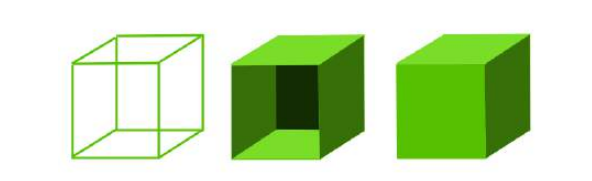
\includegraphics[width=70mm]{Dimension.PNG}
 \end{figure}
 \begin{block}{}
Dimension Hausdorff d'un espace euclidien = dimension de l'espace euclidien
\end{block}
\end{frame}

\begin{frame}{Dimension Hausdorff-Besicovitch}
\begin{block}{}
Définition en accord avec la dimension euclidienne usuelle (On peut retrouver le calcul de la dimension Hausdorff depuis le calcul de la dimension euclidienne)
\end{block}

 \begin{block}{Complexité}
    \begin{itemize}
        \item Calcul simple : autosimilarité stricte et coefficient d'homothétie constant (Flocon de Koch, Poussière de Cantor, ...)
        \item Calcul complexe et expérimental : autosimilarité approchée (Ensemble de Mandelbrot)
    \end{itemize}
\end{block}
\end{frame}

\begin{frame}{Dimension Hausdorff-Besicovitch}
Soit n le nombre de sous-ensembles obtenus lors de la réduction de facteur, et k le dénominateur du rapport homothétique $\frac{1}{k}$, alors on a la formule 1.
\begin{columns}[t]
  \begin{column}{5cm}
  \begin{block}{Formule 1}
    \begin{equation}
    d = \frac{\log n}{\log k}\label{eq:solution}
\end{equation}
Cette formule peut être retrouvée avec la formule 2
  \end{block} 
  \end{column}
  
  \begin{column}{5cm}
  \begin{block}{Formule 2}
   \begin{align*}
  E' = k^d \\
  \log(E') = \log(k^d)\\
  \log(E') = d \times \log(k) \\
  d = \frac{\log(E')}{\log(k)}
\end{align*}
  \end{block}   
  \end{column}
 \end{columns}  
\end{frame}

\begin{frame}{Dimension Minkowski-Bouligand ou "Box-counting"}
\begin{block}{}
        \begin{itemize}
        \item Méthode la plus répandue car la plus simple à utiliser
        \item Moins universel que la dimension Hausdorff-Besicovitch
    \end{itemize}
\end{block}
\begin{block}{Application}
    \begin{itemize}
        \item Imaginer ensemble fractale sur une grille régulièrement espacée
        \item Compter le nombre de boîte nécessaires pour couvrir l'ensemble
        \item Recommencer pour chaque nouvelle itération
    \end{itemize}
\end{block}
\end{frame}

\begin{frame}{Dimension Minkowski-Bouligand ou "Box-counting"}
\begin{figure}[H]
  \centering
  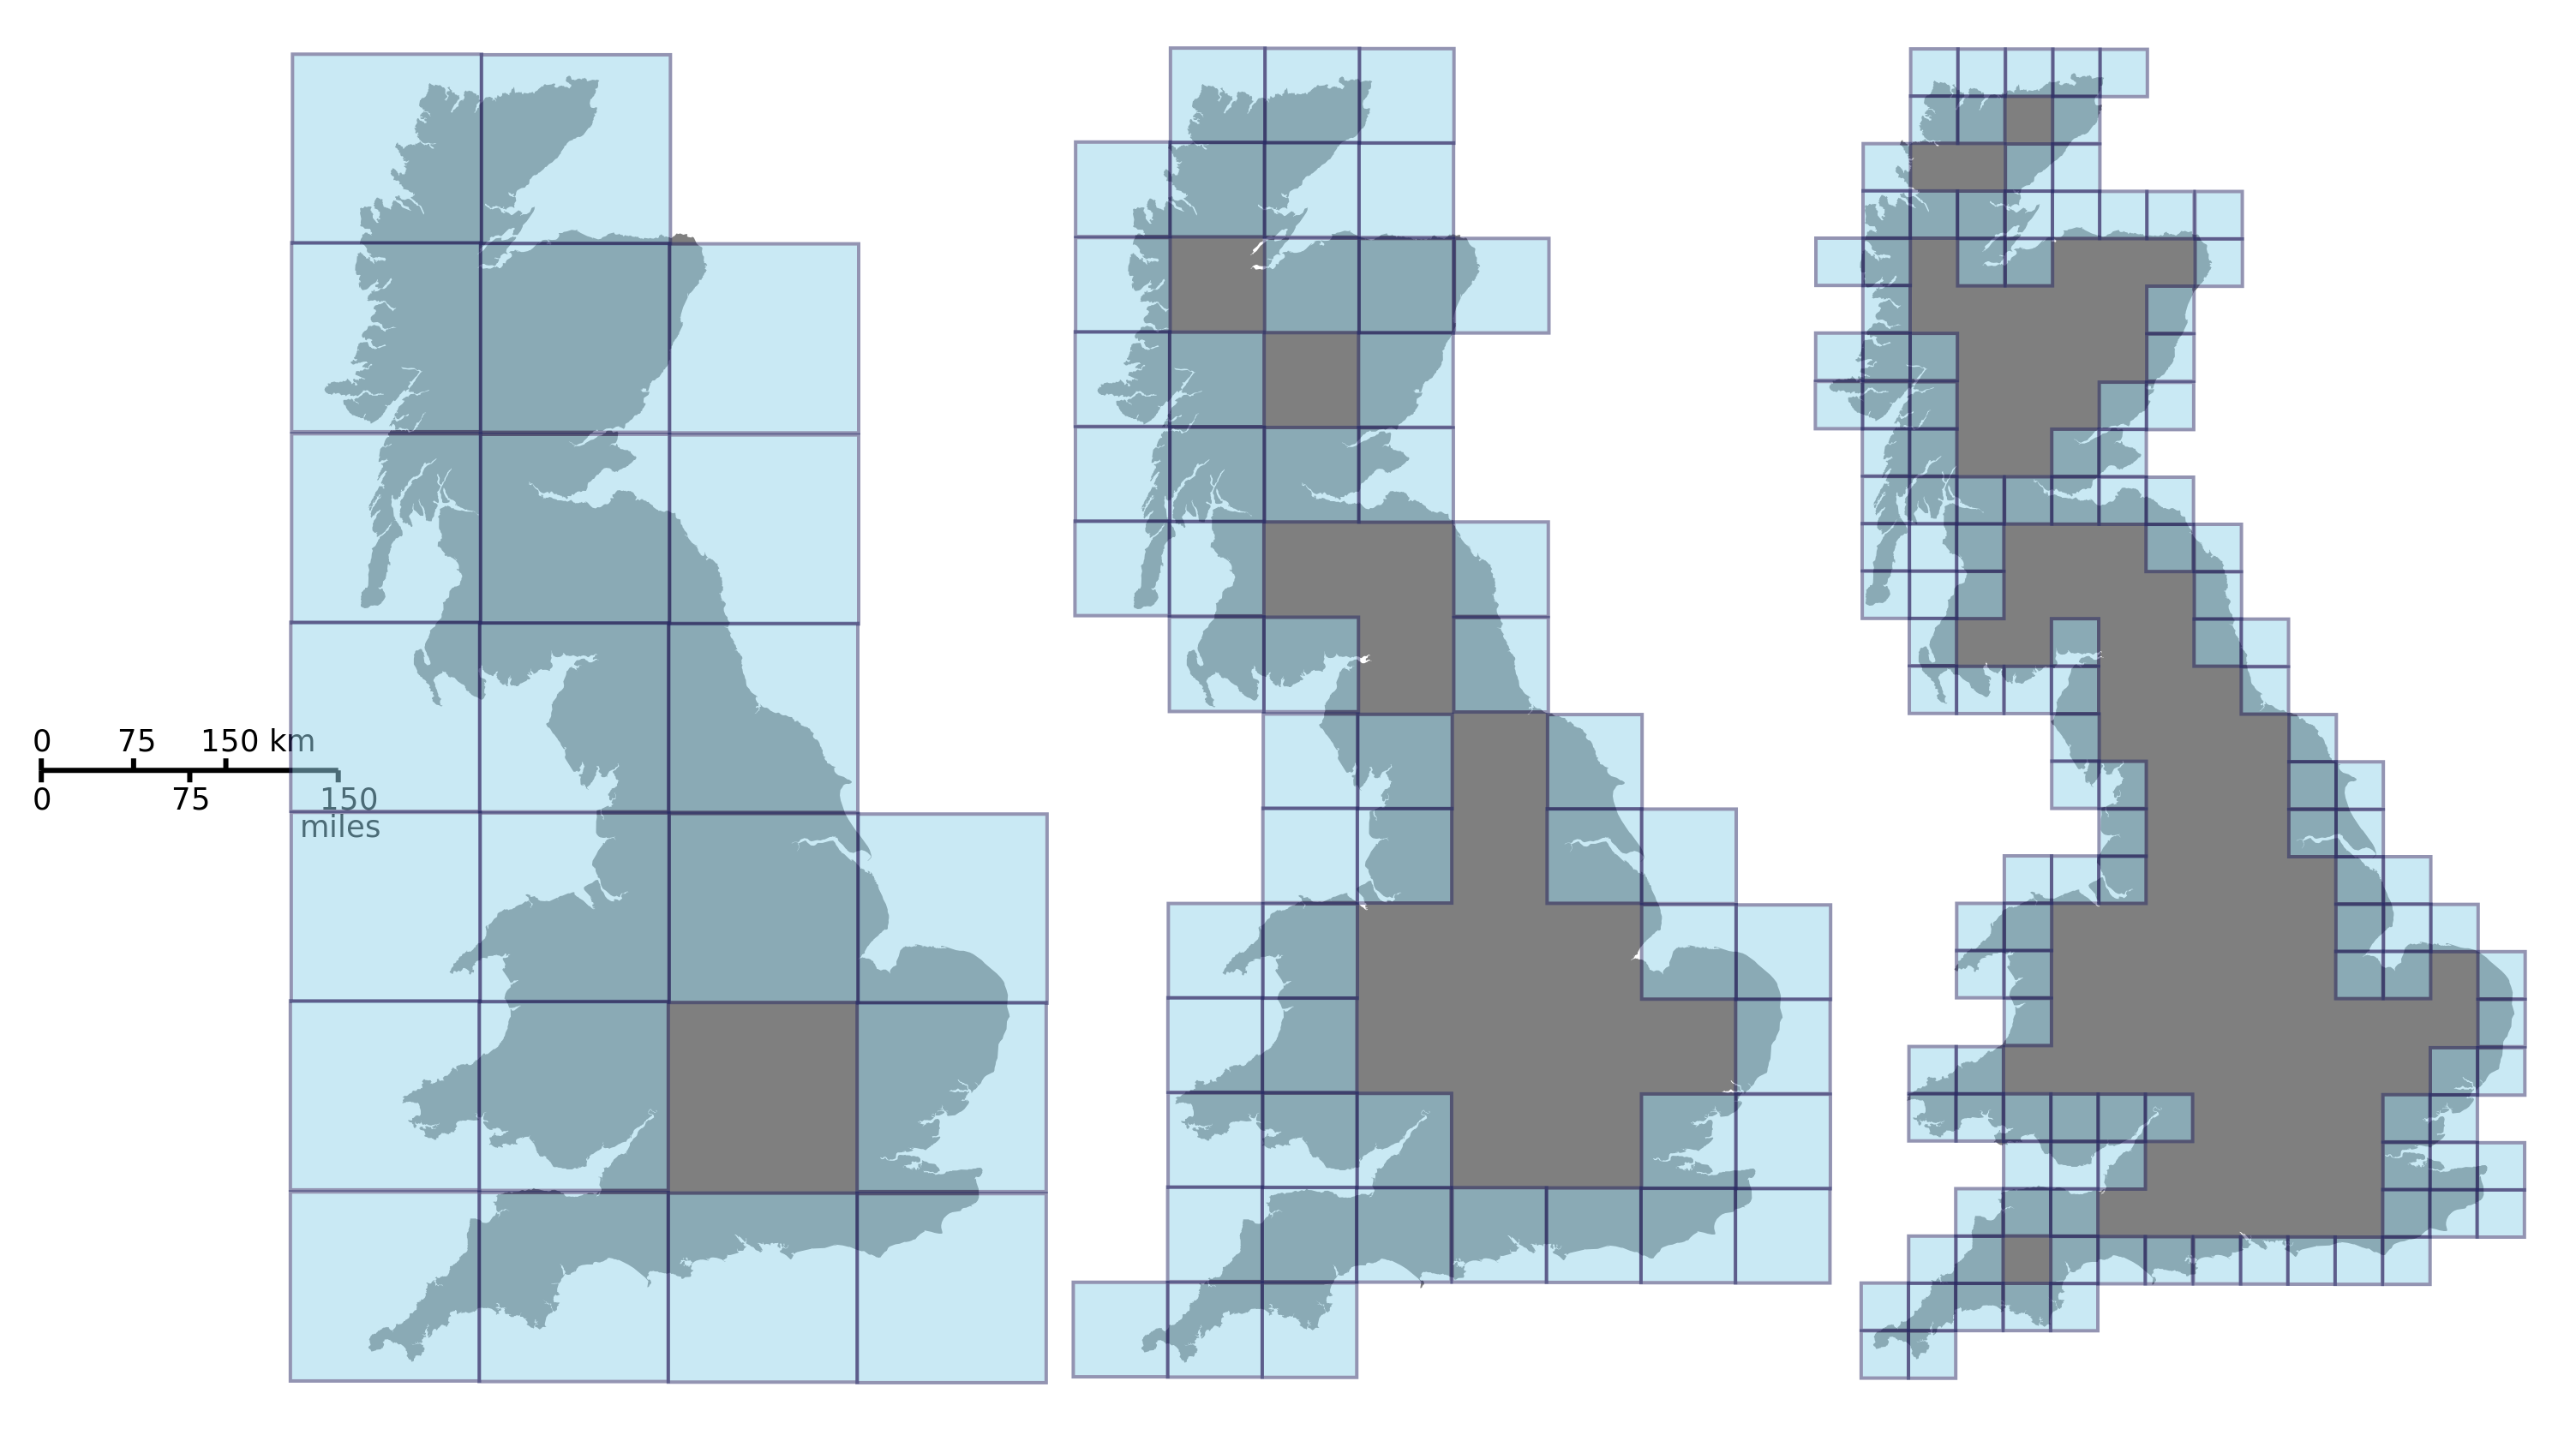
\includegraphics[width=80mm]{Great_Britain_Box.png}
 \end{figure}
\end{frame}


\section{Différentes fractales}

\begin{frame}{Flocon de Koch}
\begin{block}{}
Ensemble fractal basé sur la courbe de Koch découverte par Helge von Koch en 1904.
\end{block}
\begin{figure}[H]
  \centering
  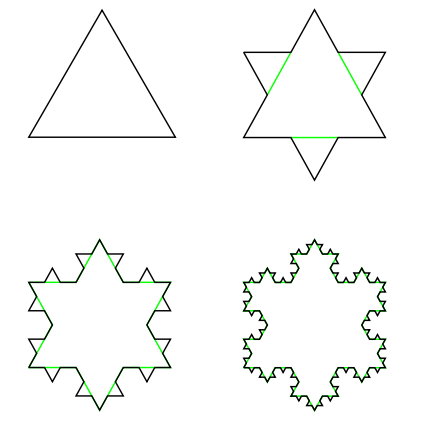
\includegraphics[width=40mm]{floncon.PNG}
 \end{figure}
\end{frame}

\begin{frame}{Flocon de Koch}
\begin{block}{Construction}
La première itération est un triangle équilatéral, récursivement chaque segment est modifié :
    \begin{itemize}
        \item On divise le segment en 3 segments de longueur égale
        \item On dessine un triangle équilatéral pointant vers l'extérieur
        \item On supprime le segment du milieu
    \end{itemize}
\end{block}
\begin{block}{Calcul de sa dimension Fractale}
    \begin{itemize}
        \item Nombre de sous-ensembles obtenu après réduction du facteur est 4
        \item Rapport d'homothétie est $\frac{1}{3}$
        \item $\frac{\log 4}{\log 3} \approx 1,261$
    \end{itemize}
\end{block}
\end{frame}

\begin{frame}{Triangle de Sierpinski}
\begin{block}{}
Ensemble fractale de la forme d'un triangle équilatéral découvert par Wacław Sierpiński
\end{block}
\begin{figure}[H]
  \centering
  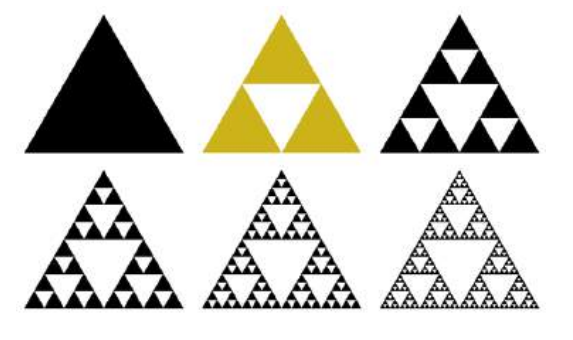
\includegraphics[width=50mm]{triangle.PNG}
 \end{figure}
\end{frame}

\begin{frame}{Triangle de Sierpinskir}
\begin{block}{Construction}
    \begin{itemize}
        \item On commence avec un triangle équilatéral 
        \item On divise le triangle en qautre triangles congruents plus petit
        \item On supprime le triangle central
        \item On recommence pour chaque triangle
    \end{itemize}
\end{block}
\begin{block}{Calcul de sa dimension Fractale}
    \begin{itemize}
        \item Nombre de sous-ensembles obtenu après réduction du facteur est 3
        \item Rapport d'homothétie est $\frac{1}{2}$
        \item $\frac{\log 3}{\log 2} \approx 1,585$
    \end{itemize}
\end{block}
\end{frame}


\section{Ensemble de Mandelbrot}
\begin{frame}{Définition}
\begin{block}{}
Ensemble représenté pour la première fois sur ordinateur par Benoît Mandelbrot en 1980.
\end{block}
\begin{columns}[t]

  \begin{column}{5cm}
  \begin{block}{Equation}
\begin{cases}
z_0=0\\
z_{n+1}=z_n^2+c
\end{cases}
  \end{block}   
  \end{column}
  
  \begin{column}{5cm}
\begin{figure}[H]
  \centering
  \includegraphics[width=50mm]{mandelbrot.png}
 \end{figure}
  \end{column}
  

 \end{columns}  





\end{frame}


\begin{frame}{Propriétés}
\begin{block}{}
    \begin{itemize}
        \item Connexité globale conjecturée
        \item Autosimilarité approchée
        \item Dimension fractale égale à 2
        \item Cardioïde et bourgeons
        \item Relation avec ensemble de Julia
    \end{itemize}
\end{block}
\end{frame}

\begin{frame}{Zoom}
\begin{block}{}
    \begin{itemize}
        \item Première image : échelle de 1
        \item Dernière image : échelle de 0.00000000005
        \item Zoom x 10 milliard
        \item Diamètre de la fractale : 4 million de kilomètres
    \end{itemize}
\end{block}
\end{frame}

\begin{frame}{Zoom}
\begin{figure}[H]
  \centering
  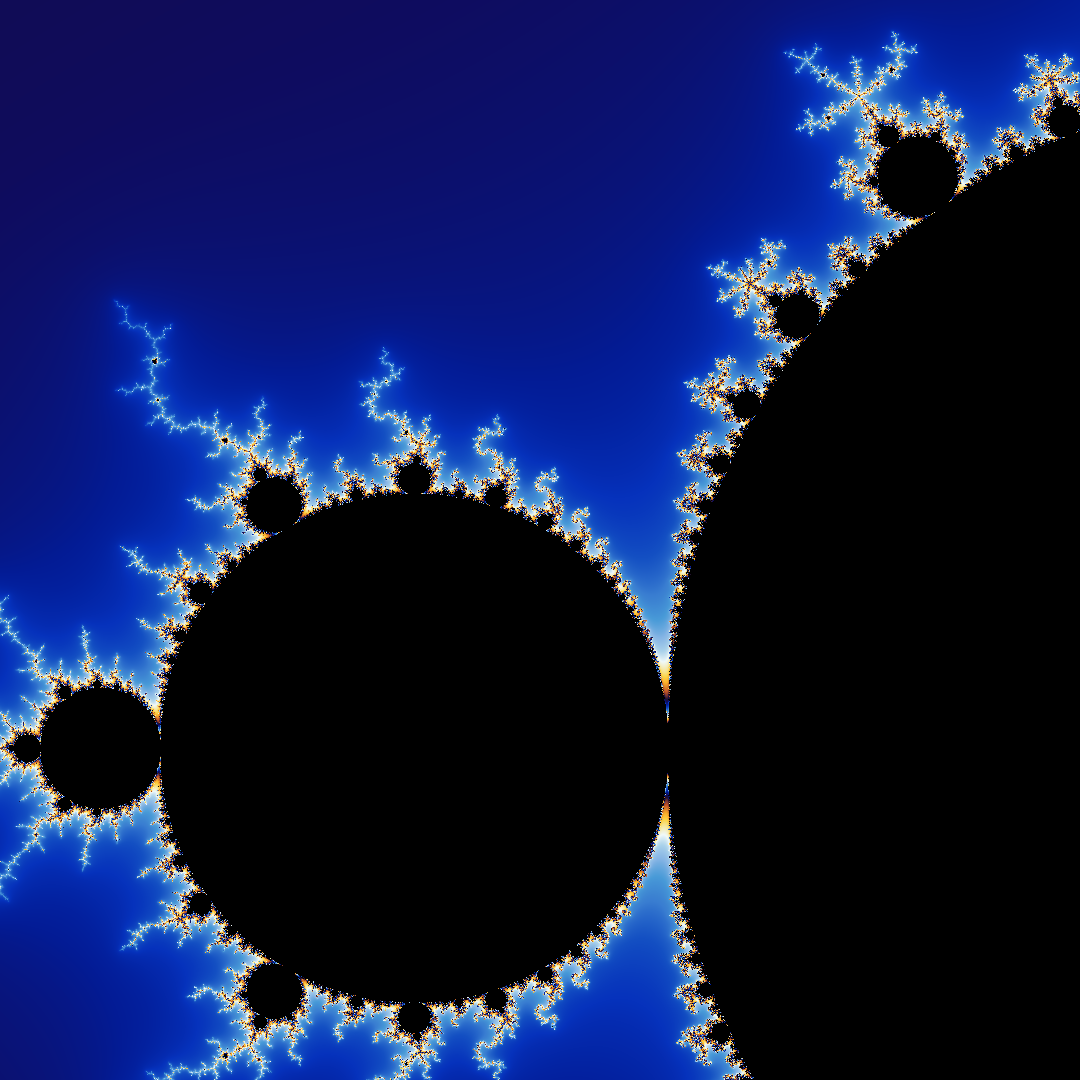
\includegraphics[width=70mm]{zoom.png}
 \end{figure}
\end{frame}

\begin{frame}{Vallée de l'hippocampe}
\begin{figure}[H]
  \centering
  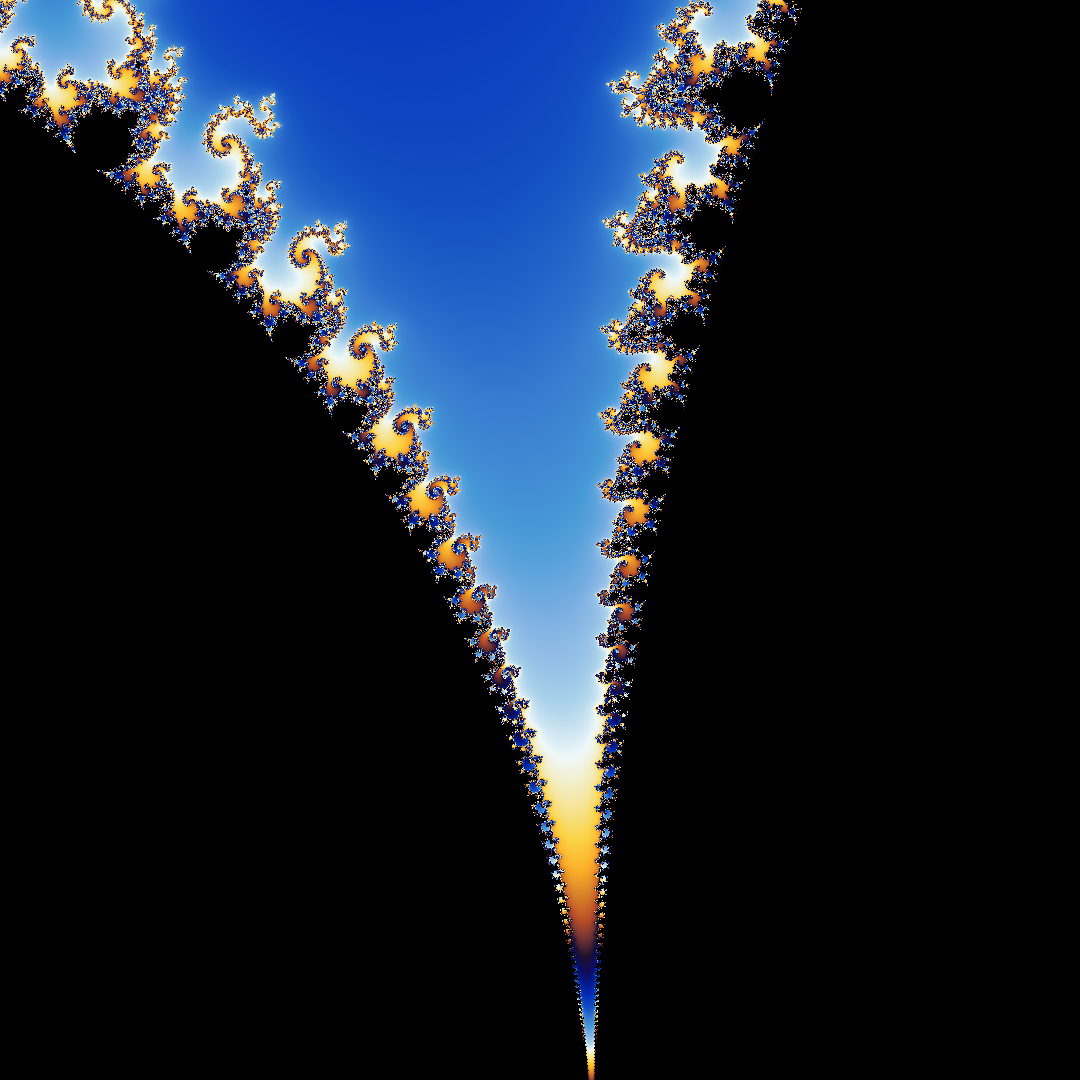
\includegraphics[width=70mm]{vallee_hippocampe.png}
 \end{figure}
\end{frame}

\begin{frame}{Hippocampe}
\begin{figure}[H]
  \centering
  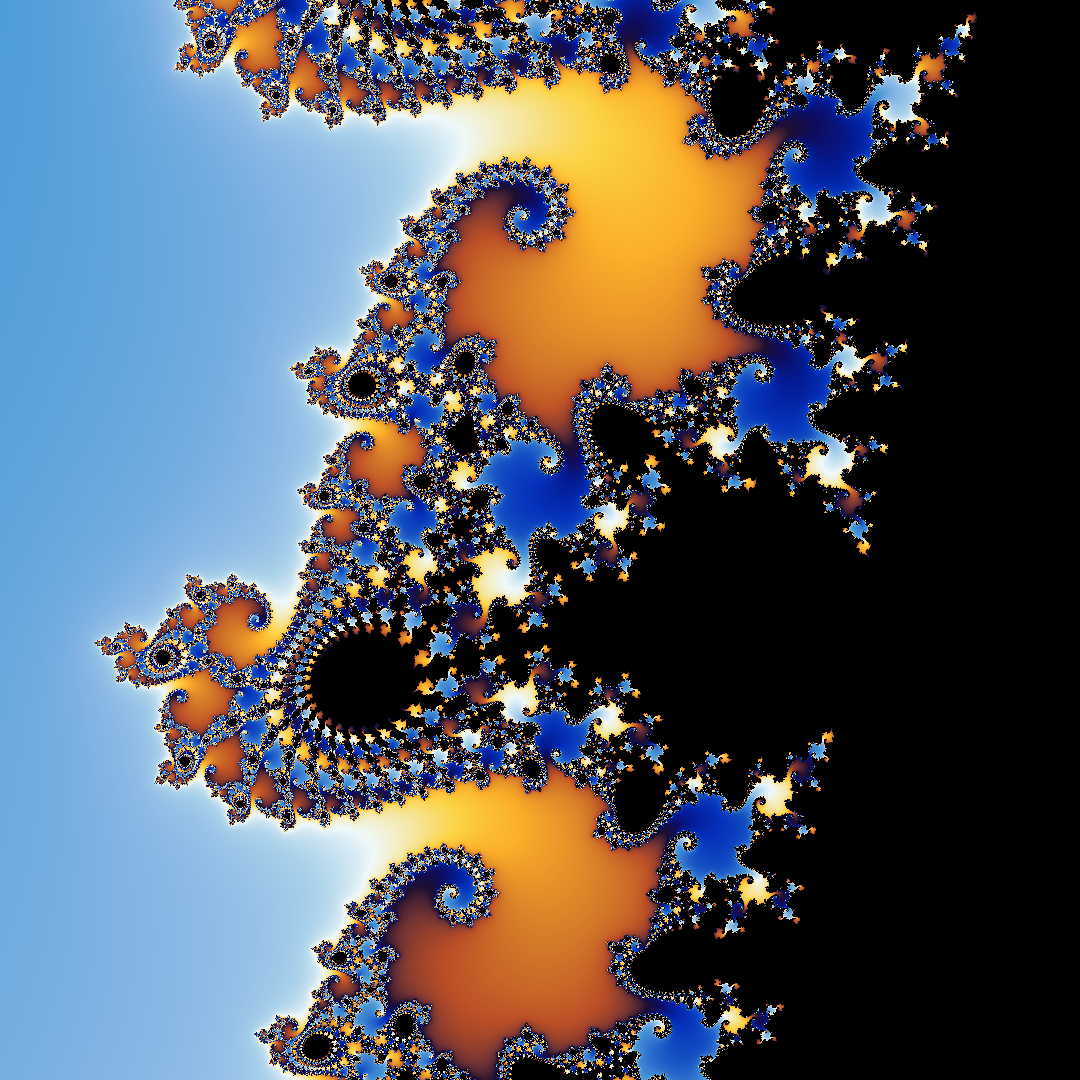
\includegraphics[width=70mm]{hippocampe.png}
 \end{figure}
\end{frame}

\begin{frame}{Queue de l'hippocampe}
\begin{figure}[H]
  \centering
  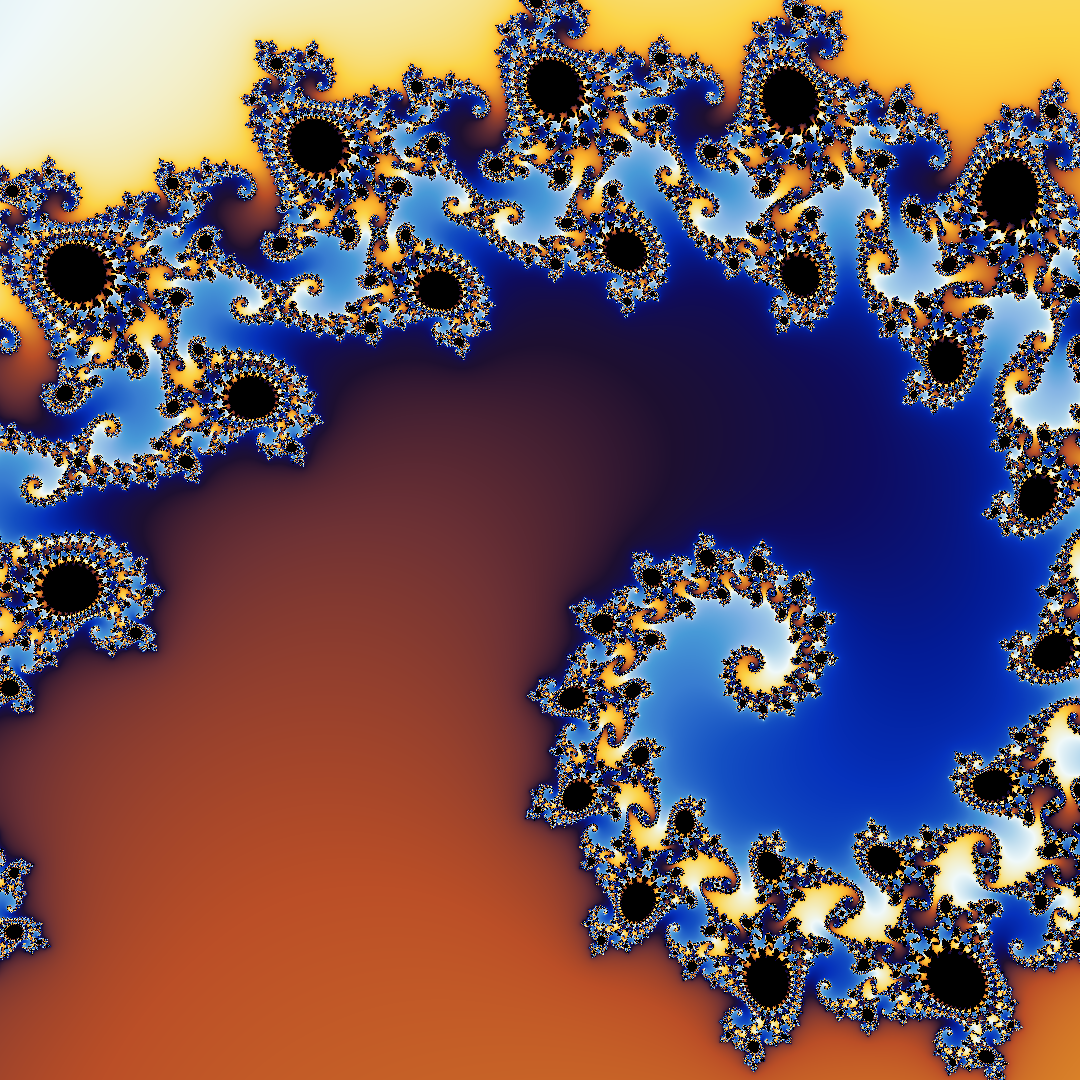
\includegraphics[width=70mm]{queue.png}
 \end{figure}
\end{frame}

\begin{frame}{Section de queue de l'hippocampe}
\begin{figure}[H]
  \centering
  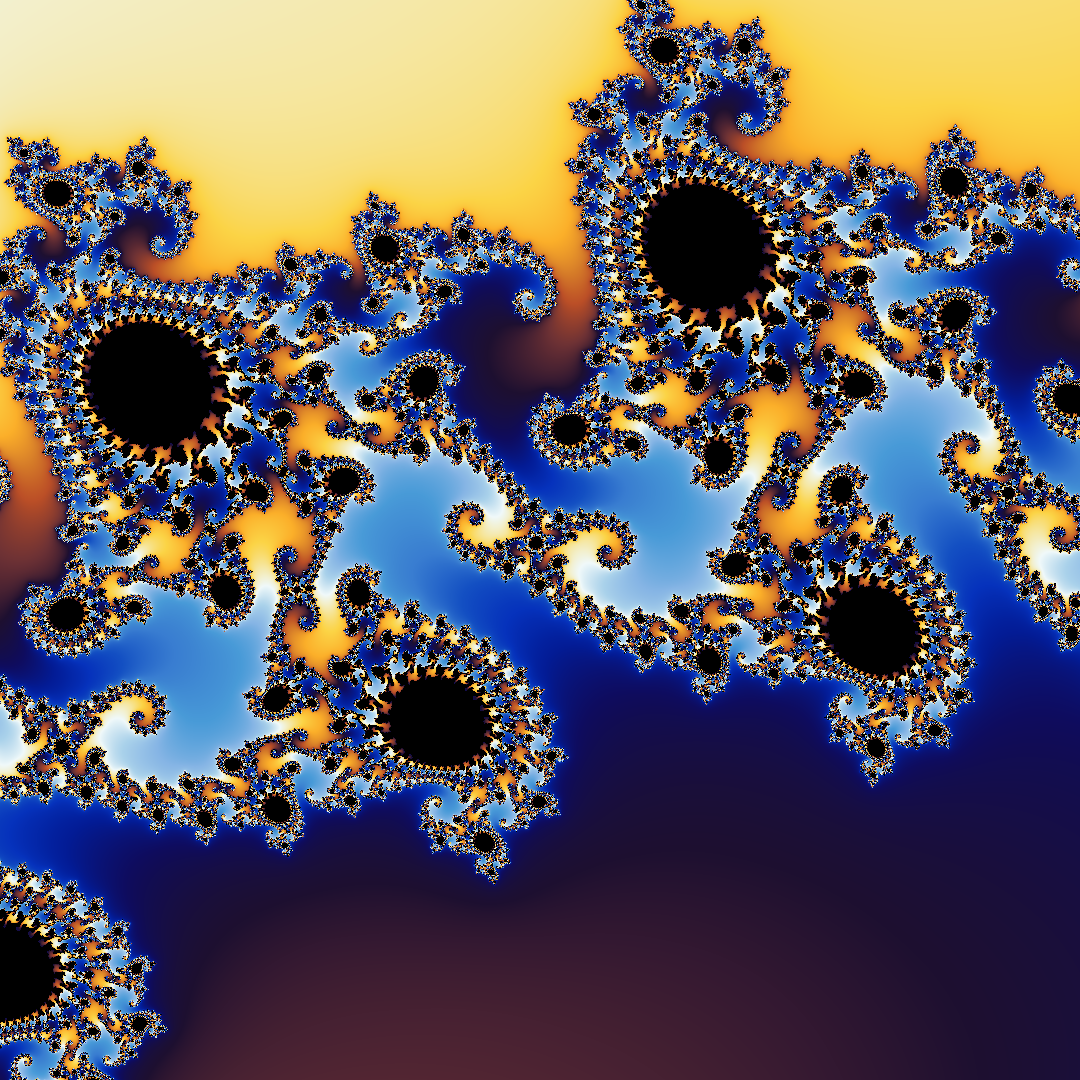
\includegraphics[width=70mm]{section.png}
 \end{figure}
\end{frame}

\begin{frame}{Satellite}
\begin{figure}[H]
  \centering
  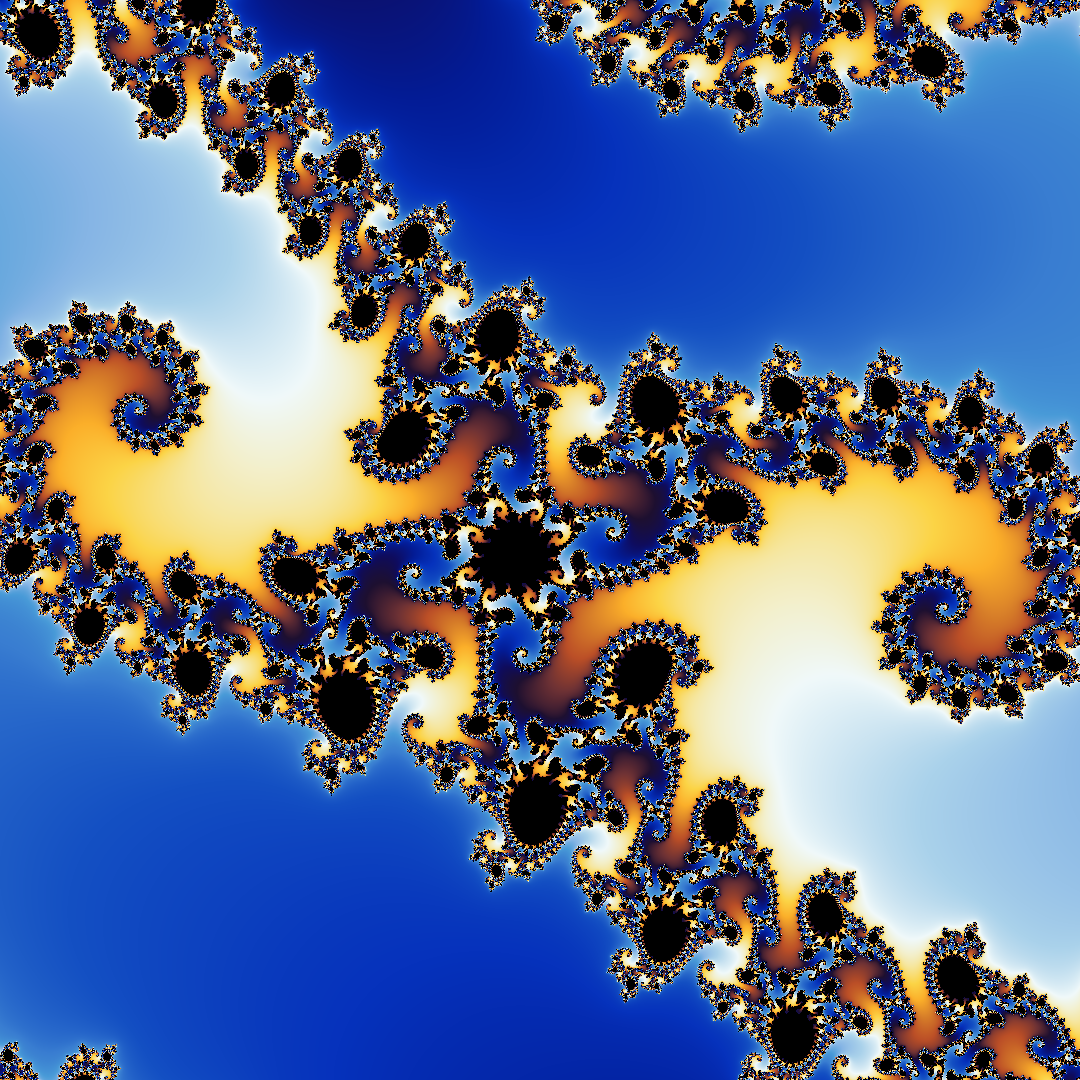
\includegraphics[width=70mm]{satellite.png}
 \end{figure}
\end{frame}

\begin{frame}{Couronne}
\begin{figure}[H]
  \centering
  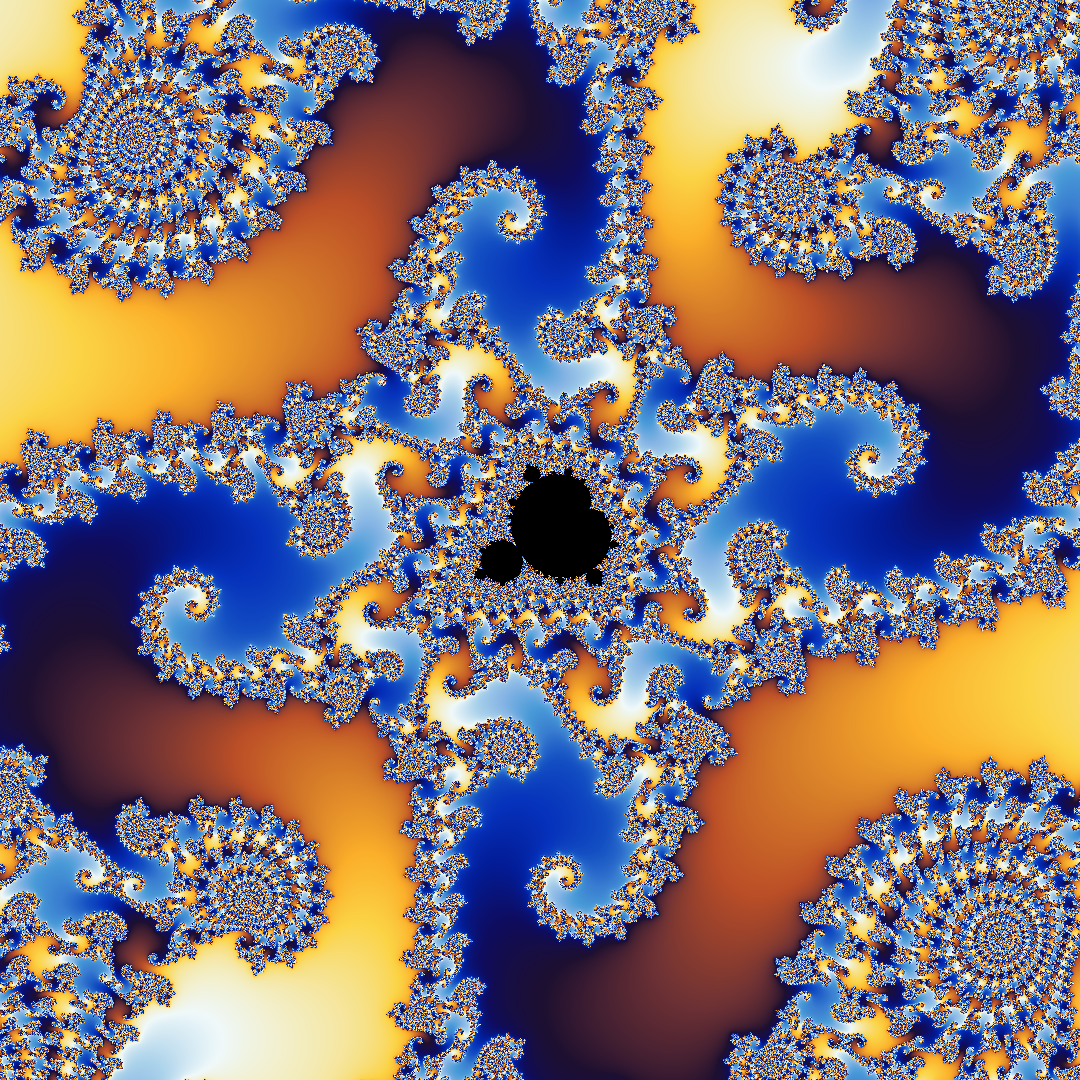
\includegraphics[width=70mm]{couronne.png}
 \end{figure}
\end{frame}

\begin{frame}{Antenne}
\begin{figure}[H]
  \centering
  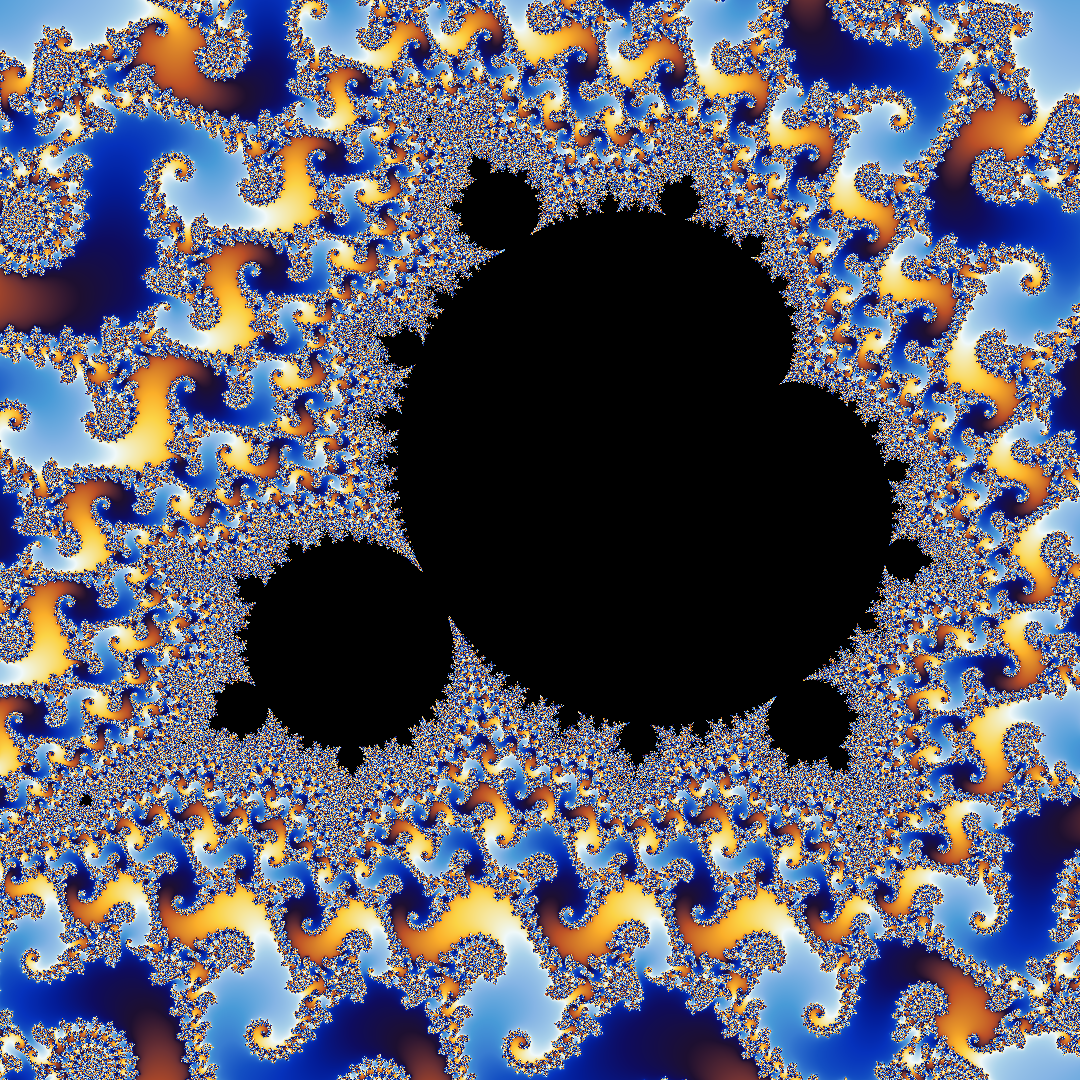
\includegraphics[width=70mm]{antenne.png}
 \end{figure}
\end{frame}

\begin{frame}{Ensemble de Julia}
\begin{figure}[H]
  \centering
  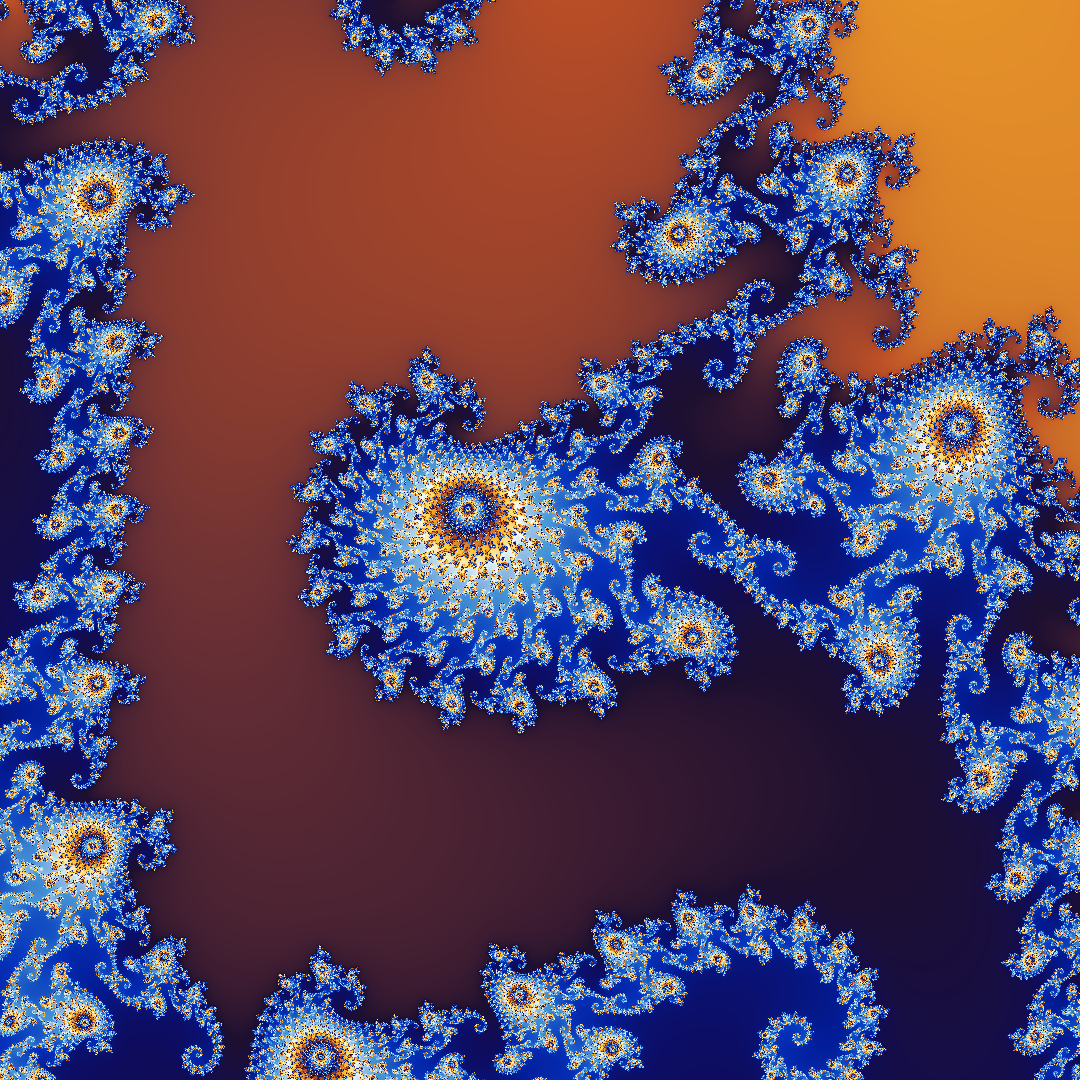
\includegraphics[width=70mm]{julia.png}
 \end{figure}
\end{frame}

\begin{frame}{Îlot}
\begin{figure}[H]
  \centering
  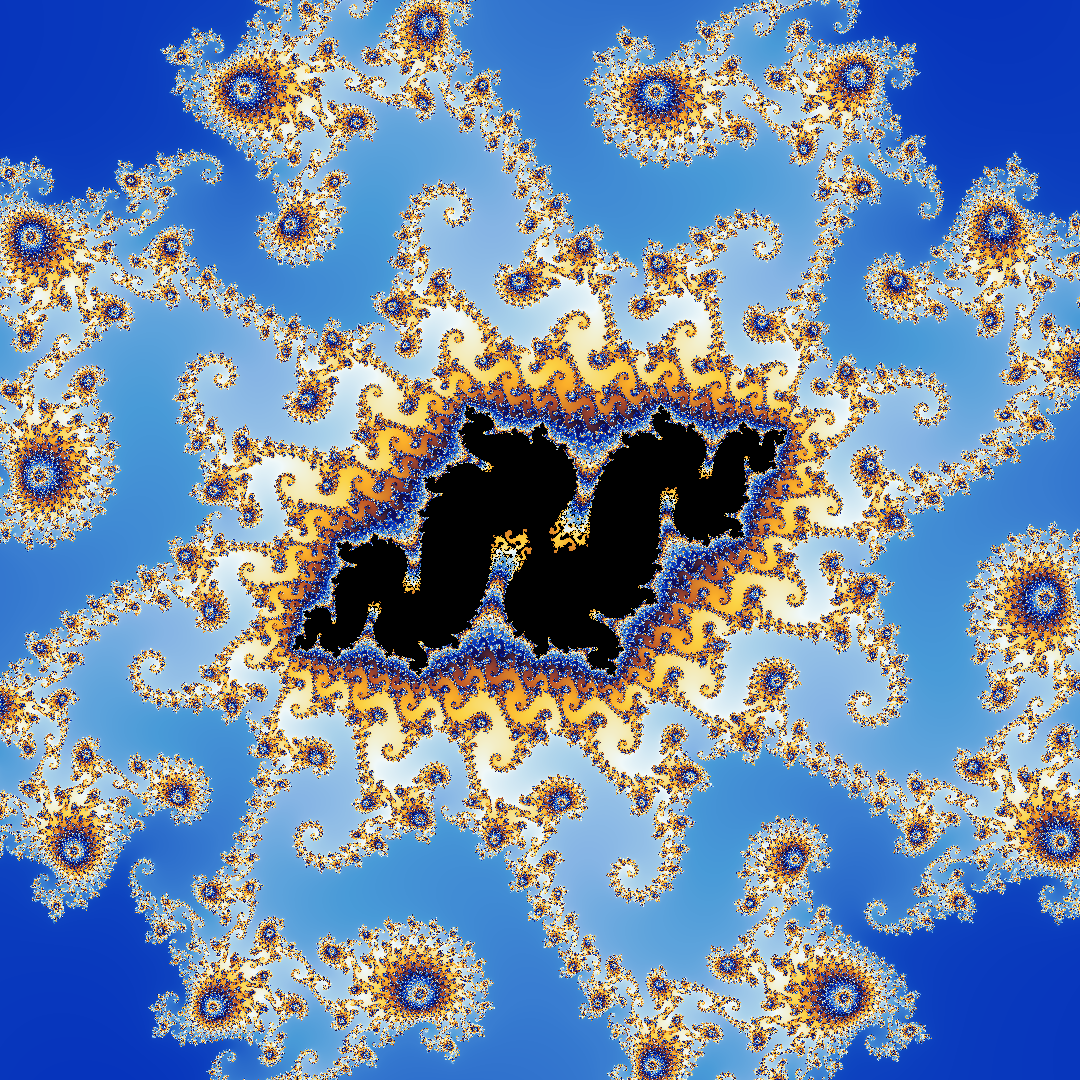
\includegraphics[width=70mm]{ilot.png}
 \end{figure}
\end{frame}

\section{Génération}
\begin{frame}{Escape-time}
\begin{block}{}
    \begin{itemize}
        \item Calcul effectué pour chaque point de coordonnée (x, y)
        \item Couleur attribuée selon le résultat du calcul
        \item Valeurs vérifiées à chaque itération 
        \item "Escape" ou "Bailout" : valeur cohérente avec le système
        \item Nombre maximum d'itération
    \end{itemize}
\end{block}
\end{frame}

\begin{frame}[fragile]{Implémentation}
  \begin{verbatim}
for(int pX=0; pX < dimensionX; pX++){
    for(int pY=0; pY < dimensionY; pY++){
        x0 = (cX - Rayon) + (2* rayon * pX)/dimensionX;
        y0 = (- cY - Rayon) + (2* rayon * pY)/dimensionY;
        while (x*x + y*y <= 2*2  && iteration < max) {
            temp = x*x - y*y + x0
            y = 2*x*y + y0
            x = xtemp
            iteration = iteration + 1
        }
        color = palette[iteration]
        setColor(Px, Py, color)
    } 
}

   \end{verbatim}
\end{frame}

\begin{frame}{Implémentation}
\begin{block}{}
    \begin{itemize}
        \item C++
        \item Image pixmap (.ppm)
        \item Palette de couleurs
        \item Escape-time : fonctionne mais esthétiquement étrange
        \item Normalized iteration count corrige ce problème
        \item Utilisation de thread
    \end{itemize}
\end{block}
\end{frame}

\section{Conclusion}
\begin{frame}{Conclusion}
\begin{block}{}
    \begin{itemize}
        \item Sujet vaste et complexe
        \item Nombreux domaines d'applications
        \item Recherche stagnante
        \item Représentation visuelle de plus en plus grande
        \item Dimension Hausdorff de l'ensemble de Mandelbrot
    \end{itemize}
\end{block}
\end{frame}

\end{document}

